
\section{Hall-B Beamline Design}
\label{beamlinedesign}

As was described in Ref.~\cite{HPSBeamline}, the Hall B beamline is divided into two segments, the so-called ``2C" line from the Beam 
Switch Yard (BSY) following beam extraction from the CEBAF accelerator to the hall proper, and the ``2H" line from the upstream end of 
the experimental hall to the beam dump in the downstream tunnel. The beamline upstream of CLAS12 is furnished with a number of 
quadrupoles, corrector dipoles, and beam diagnostic tools, grouped into sections. Accelerator operators have exclusive control of these 
devices and use this instrumentation to tune and deliver the beam to the CLAS12 target located approximately at the geometrical center of the 
hall. In addition to the devices used by accelerator operations, there are several beam position, current, polarization, and halo monitors that 
are controlled and monitored by Hall-B shift personnel. 

For high-energy operation of CLAS12, the 2C beamline as described in Ref.~\cite{HPSBeamline} was modified to include 
the M{\o}ller polarimeter located in the upstream tunnel of the hall %(see Fig.~\ref{fig:upstream})
 and an intermediate beam dump just upstream 
of the hall. Additionally, the 2H beamline (Fig.~\ref{fig:hall1}) now includes a cryogenic target and a tungsten shield downstream of the 
target inside the CLAS12 torus magnet bore. The M{\o}ller polarimeter is used to periodically measure the longitudinal beam polarization and is discussed in more detail in Sec.~\ref{mollerpol}.  The other components are discussed immediately below.

% had to move this figure to intro section so that it would end up where I wanted it
%\begin{figure*}[t]
%\begin{center}
%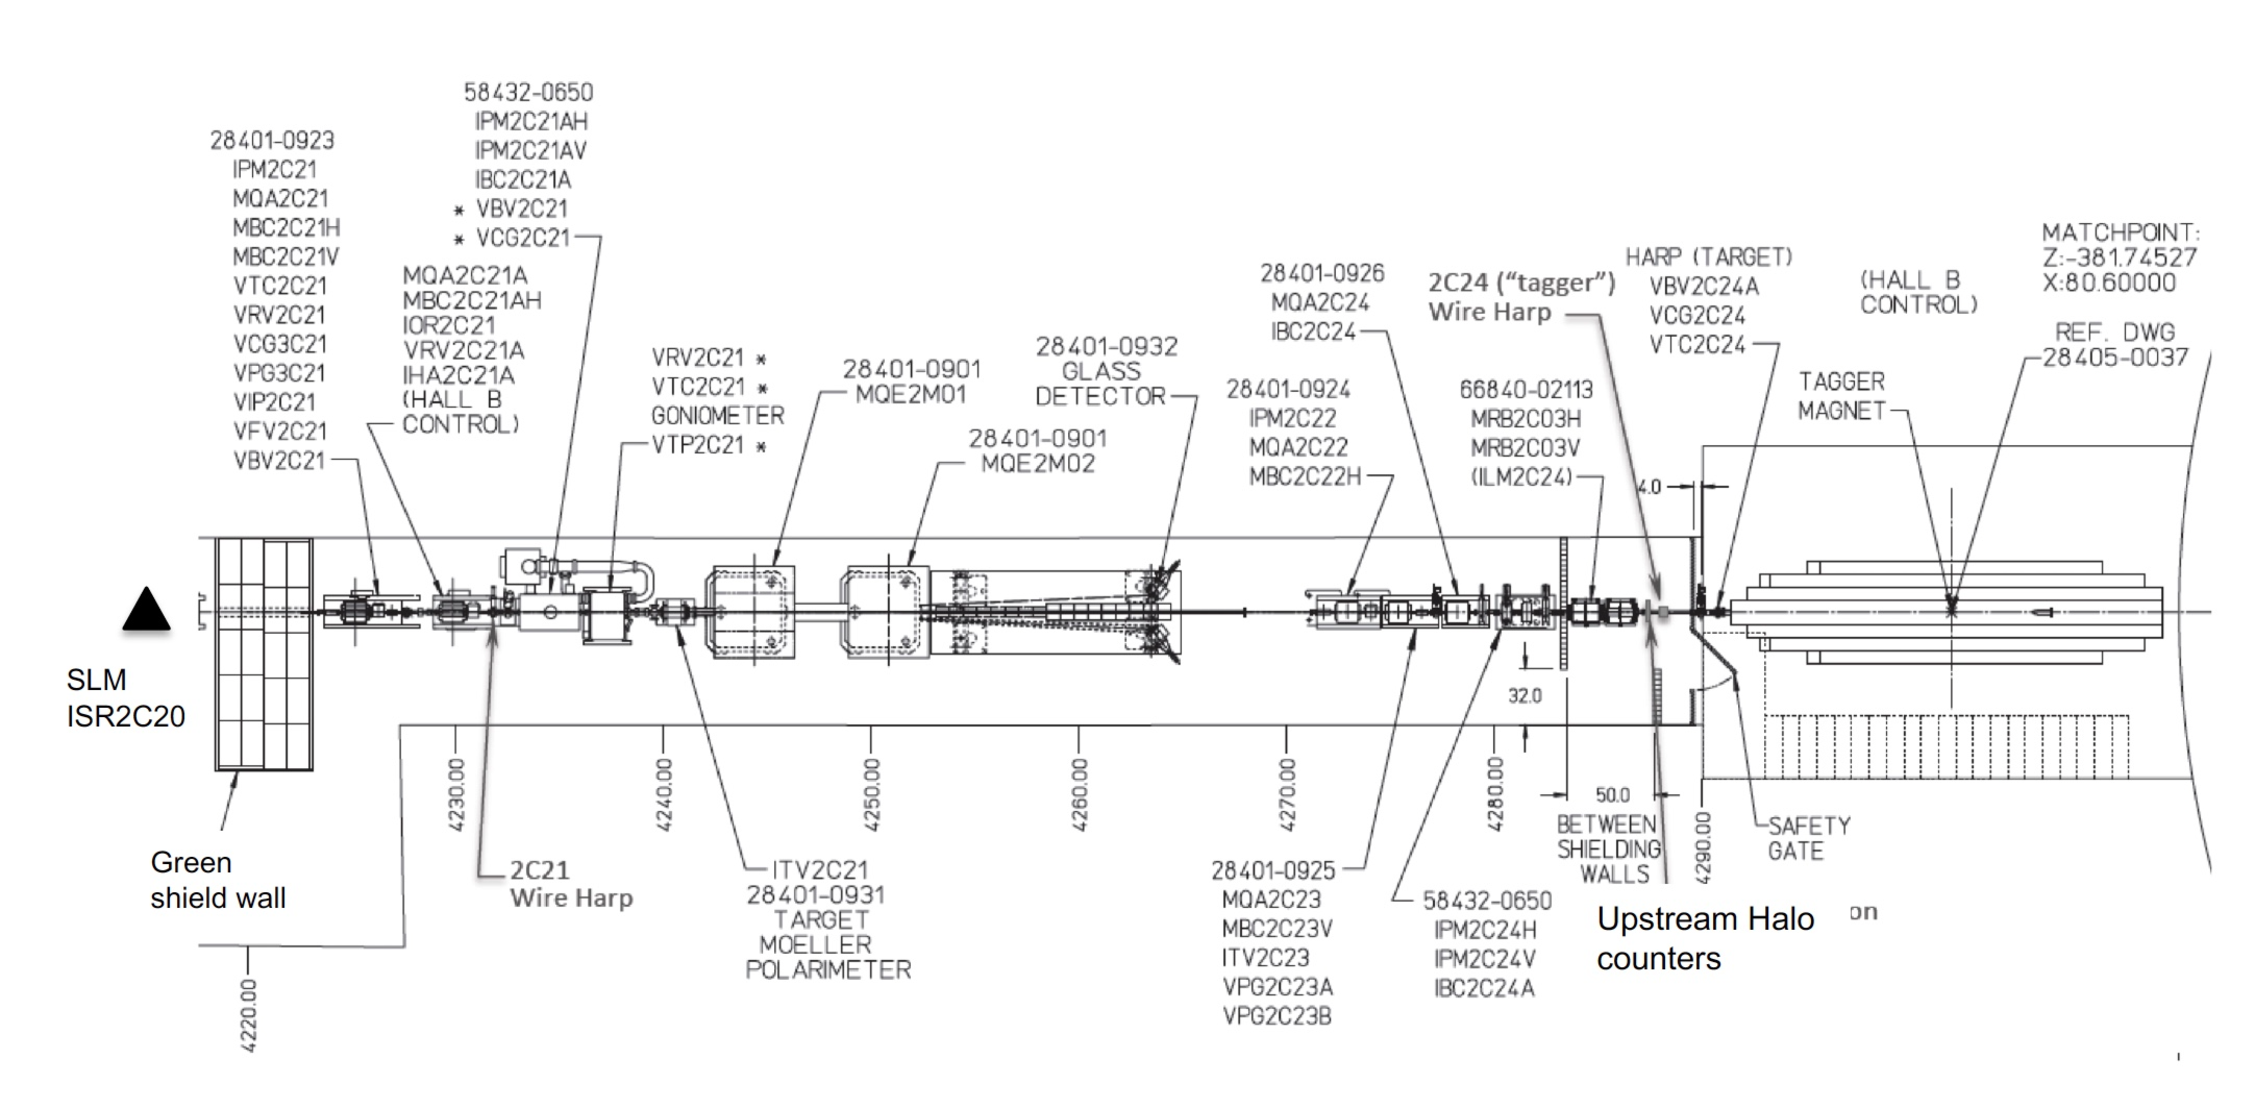
\includegraphics[width=1.\textwidth]{upstream_tunnel.pdf}
%\caption{Overhead view of the 2C beamline in the tunnel upstream of Hall B. {\color{red} Not the final figure.}}
%\label{fig:upstream}
%\end{center}
%\end{figure*}

\begin{figure*}[t]
\begin{center}
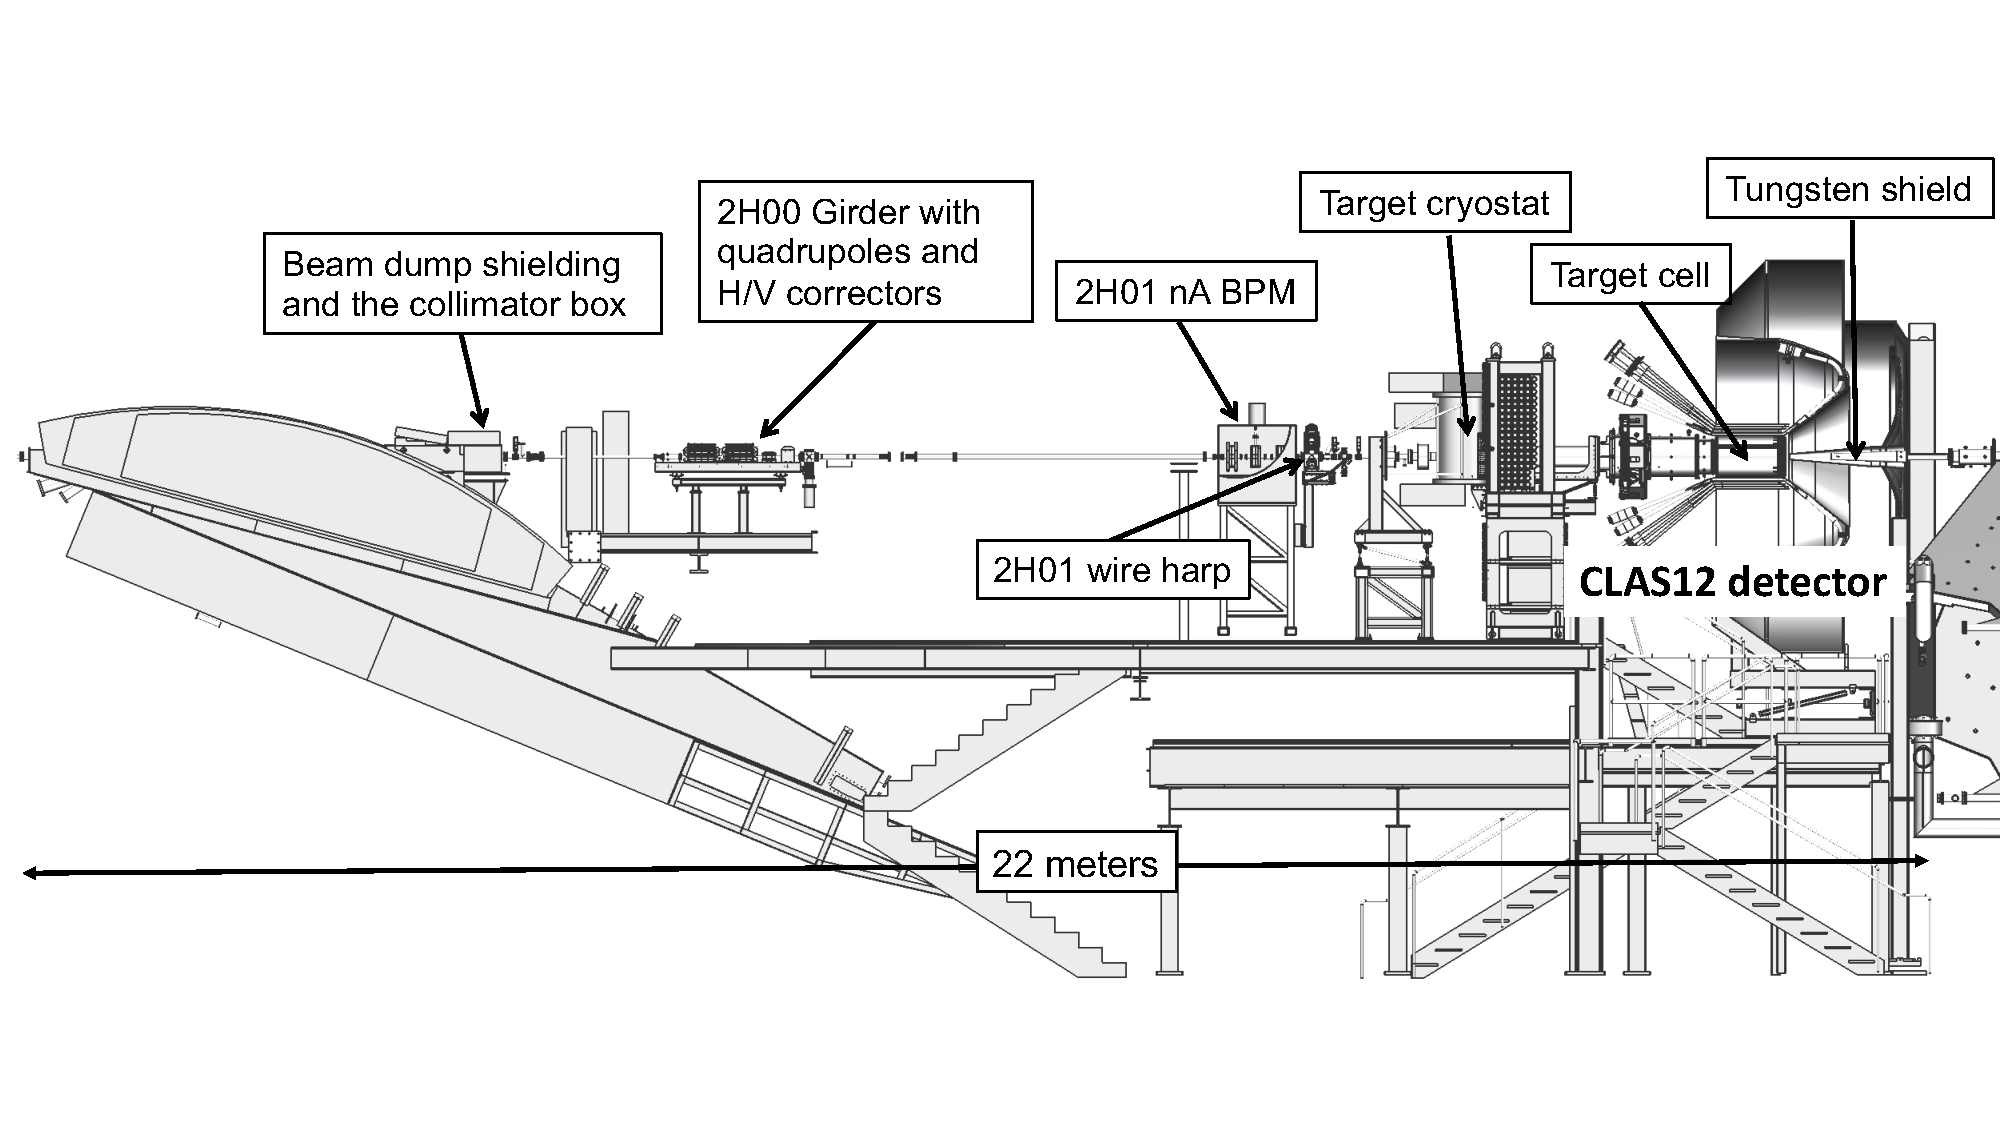
\includegraphics[width=1.\textwidth]{beamline_hall_1.pdf}
	\caption{Beamline in Hall B showing beamline elements upstream of the CLAS12 target, cryotarget, CLAS12 central detector and 
	the tungstem shield downstream of the scattering chamber.}
\label{fig:hall1}
\end{center}
\end{figure*}


\subsection{Intermediate beam dump before CLAS12}
\label{sec-IBD}

In order to prevent radiation damage to the sensitive detectors during the initial beam tune, or when errant beam may be sent to the hall, 
or during the beam polarization measurements with the M{\o}ller polarimeter, the beam has to be terminated upstream of CLAS12. For these 
operations the Hall-B tagger dipole magnet is used to deflect the primary beam and secondary scattering products. During low-energy 
operations, the tagger dipole directs the beam into the tagger beam dump in the hall floor upstream of the CLAS12 spectrometer. The highest 
energy beam that can be directed to this dump is limited to $6.2$ GeV by the maximum field of the tagger dipole, 
1.76 T \cite{tagger}. At higher energies, a few options for the intermediate beam dump were considered during the design stage with 
the optimal solution being to dump the beam inside the bore of the tagger magnet yoke. The design of the intermediate dump was based on
full FLUKA \cite{fluka} simulations and on thermal finite-element analysis. The two main parameters that were studied were the radiation levels at 
the location of the CLAS12 tracking detectors and the temperature rise in the magnet yoke when up to 10 nA of continuous wave (CW) 
electron beam is dumped on the yoke.  

The FLUKA simulations were used to determine background radiation levels at the tracking detectors for different configurations of the 
dump and compared with radiation levels from various targets and beam currents at the design luminosity.  It was found that acceptable 
background radiation levels from the dump occur when the beam is steered into the yoke at approximately 33 cm from the upstream 
entrance to the tagger magnet bore, as shown in Fig.~\ref{fig:yokedump}. This is done by setting the tagger magnetic field to be 
$I({\rm A}) = 43.491\times E({\rm GeV}) - 0.076$, where $I$ and $E$ are 
the tagger power supply current and the beam energy, respectively.   
%
\begin{figure}[hbt]
\begin{center}
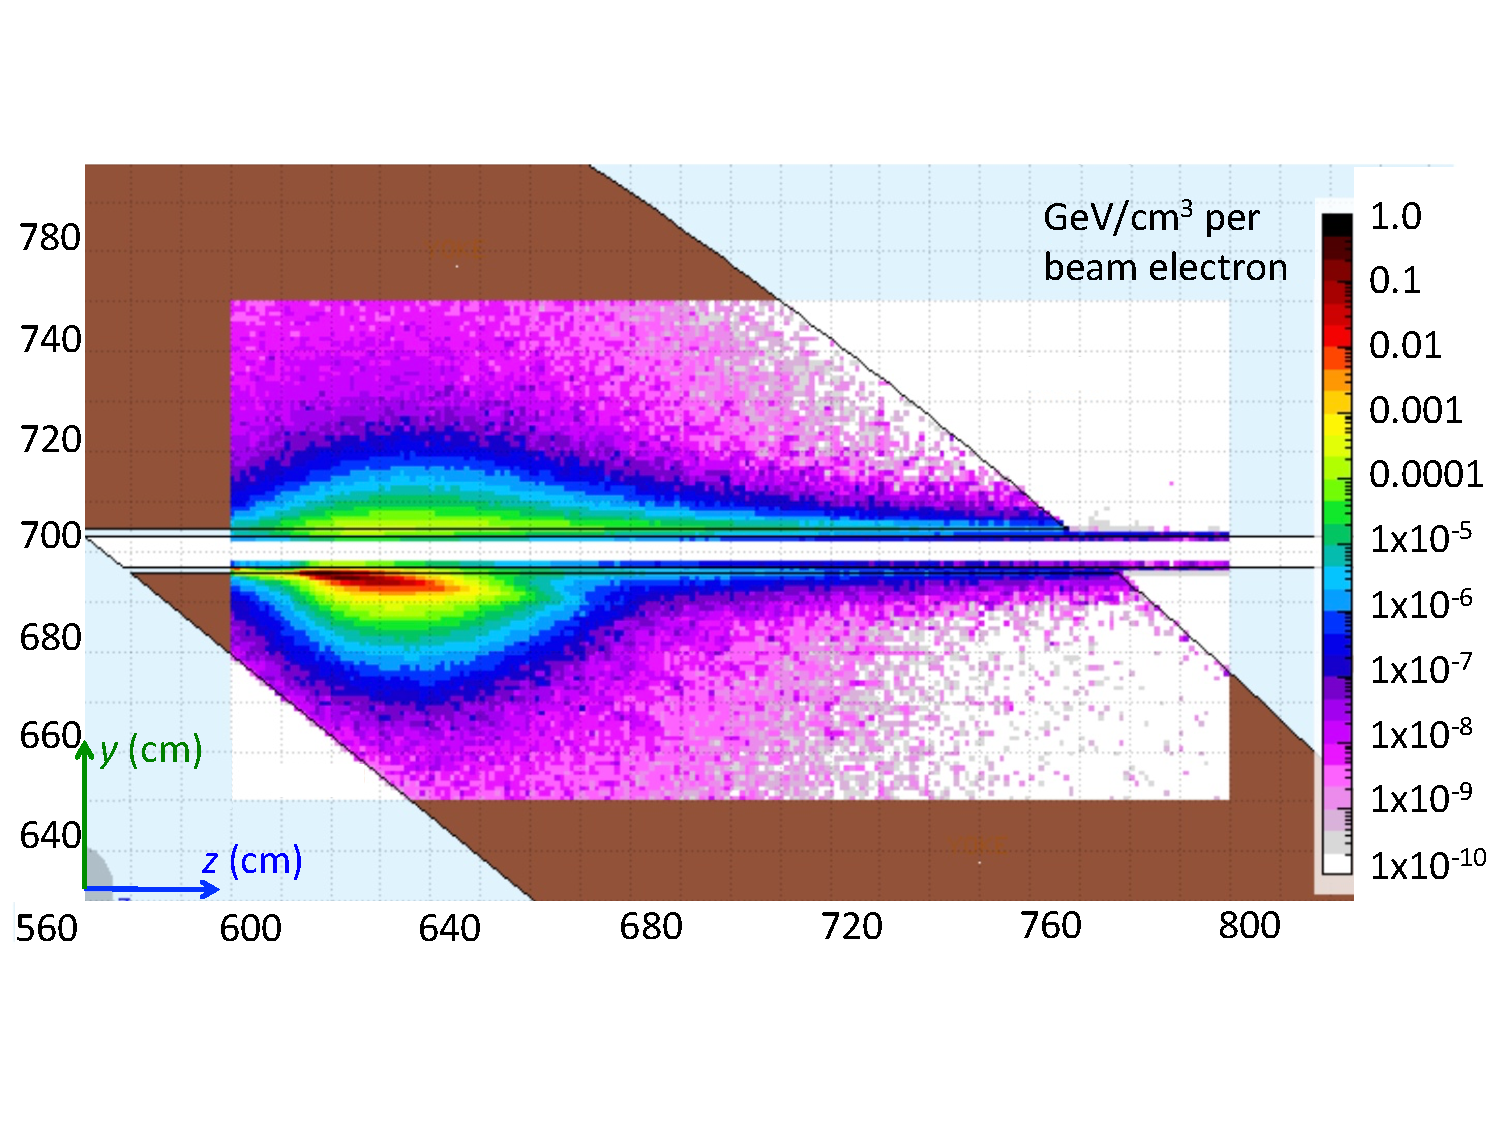
\includegraphics[width=.45\textwidth]{YokeDump.pdf}
	\caption{Distribution of energy in the yoke of the tagger dipole magnet from dumping a 10 nA, 11 GeV beam on the yoke at 
	$\sim33$ cm from the upstream entrance to the bore of tagger. Horizontal and vertical scales are distances in cm and energy 
	deposition (in GeV/cm$^3$) is indicated by the color scale. The brown region indicates the cross section of the tagger yoke.}
\label{fig:yokedump}
\end{center}
\end{figure}

The FLUKA simulations were also used to guide the design of the shielding around and just downstream of the tagger magnet yoke. 
The shielding includes lead, borated polyethylene, and concrete blocks. Figure~\ref{fig:raddem} shows the 1-MeV neutron equivalent 
fluency for the background from the dump and for various beam/target configurations as a function of the position along the beamline. 
In the graph, the yoke dump position is at approximately -900 cm and the CLAS12 target is at $\sim400$ cm. The figure shows that at 
the location of the CLAS12 target, the designed shielding configuration (filled black points) results in radiation levels from the yoke 
comparable to levels for running on a carbon target at the full design luminosity.   

\begin{figure}[hbt]
\begin{center}
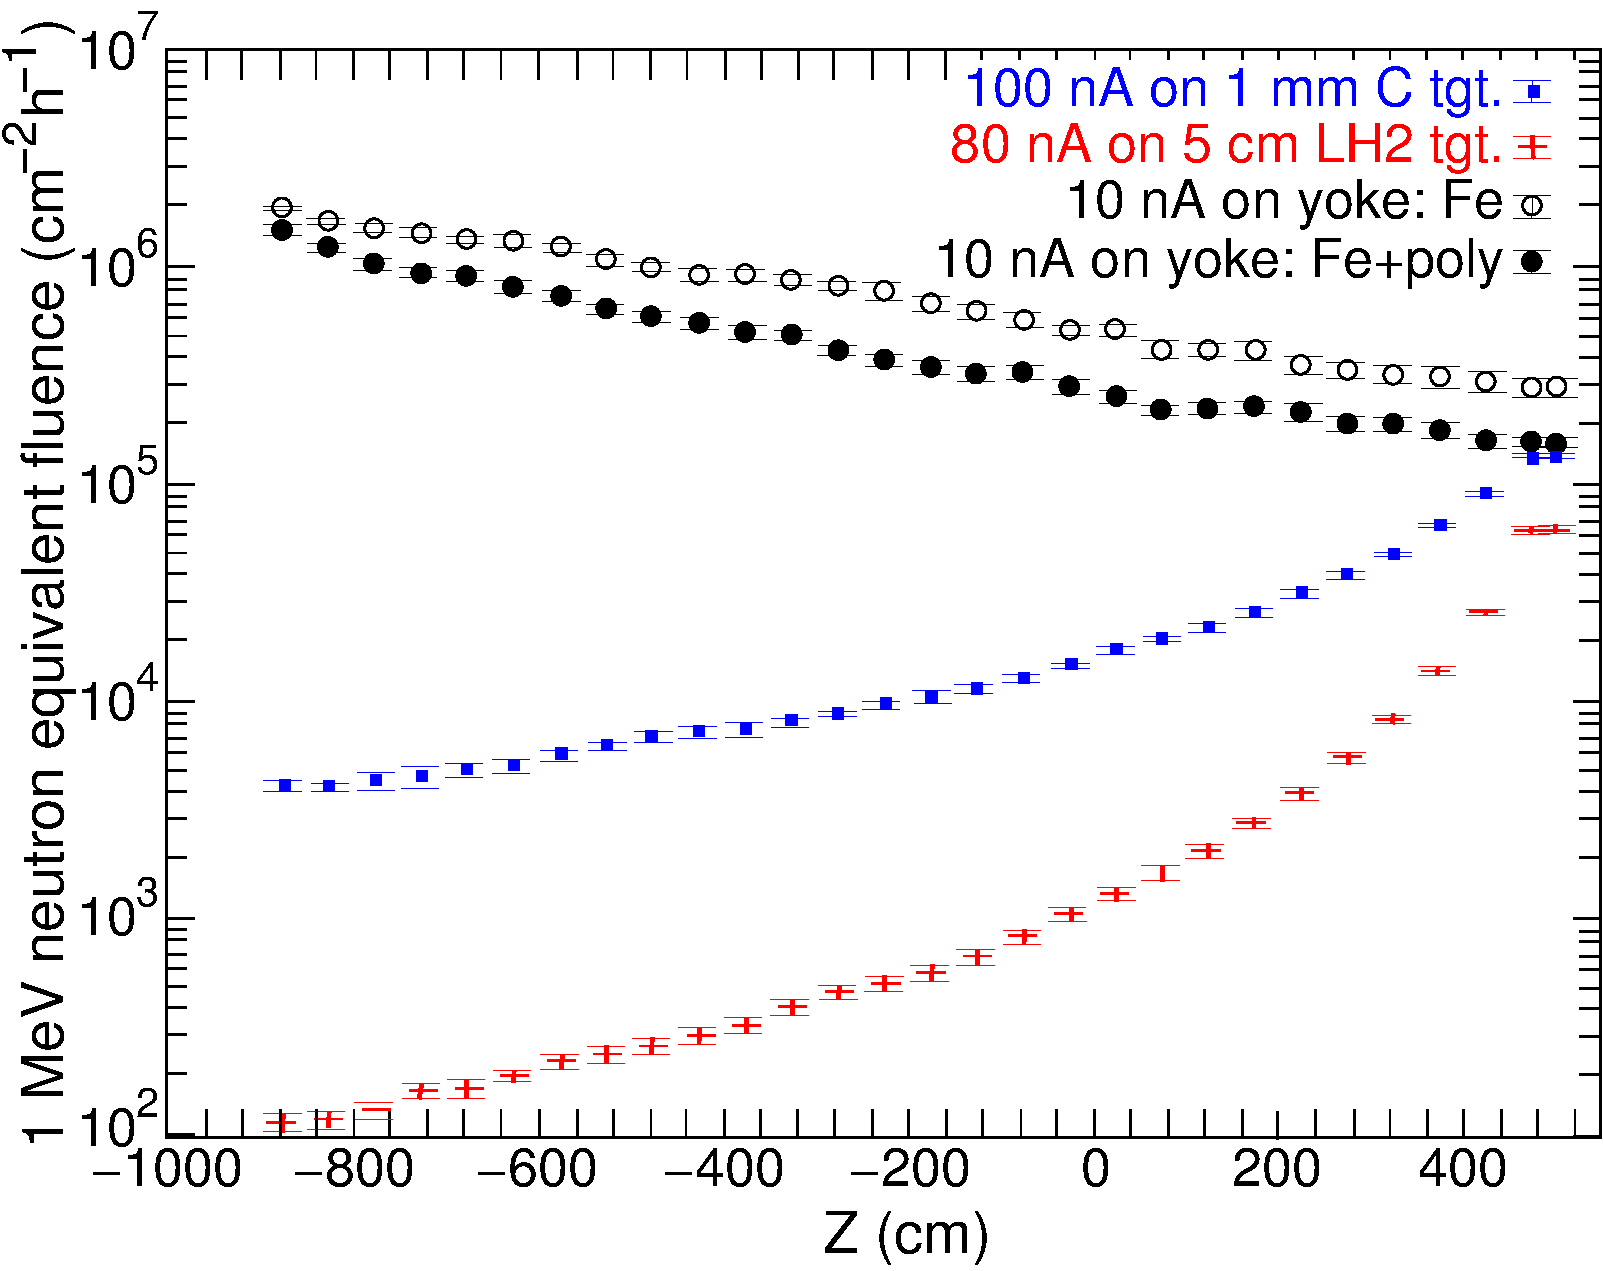
\includegraphics[width=0.45\textwidth]{Radiation.pdf}
%\includegraphics[width=0.45\textwidth]{radiation_hadrons.pdf}
	\caption{FLUKA simulation of radiation levels in the hall from dumping a 10 nA, 11 GeV beam on the tagger magnet yoke compared to 
	the radiation levels from nominal running on hydrogen and carbon targets. The 1-MeV neutron equivalent fluency as function of position along the beamline for yoke shielding with iron only, open circles, and with iron and borated polyethylene, filled circles, and for two target configurations, 1 mm carbon, filled squares, and 5 cm long liquid hydrogen, crosses.}
\label{fig:raddem}
\end{center}
\end{figure}

To assess the temperature increase in the yoke, a thermal finite-element analysis was set up using ANSYS Workbench v18 \cite{ANSYS}. 
A simplified CAD model of the yoke was imported and modified to include a cylindrical heat load representing the beam. The heating 
profile from the deposition of 1 kW of power in a cylinder of one Moliere radius ($r = 1.7$ cm) and 10 radiation lengths (17 cm) of iron 
was calculated. Conservatively, adiabatic boundary conditions were applied to the outer surfaces of the yoke. The model was solved as 
a transient thermal analysis with 100 time points over 3600 seconds. At the dump location, the temperature was found to initially increase
rapidly and then stabilized to a maximum temperature increase of $\Delta T = 54^\circ$C as the heat dissipates throughout the yoke 
volume (see Fig.~\ref{fig:ansys_yoke}). Due to the very large volume and heat capacity of the yoke, the temperature is not expected to 
rise much higher even for longer beam application times.

\begin{figure}[hbt]
\begin{center}
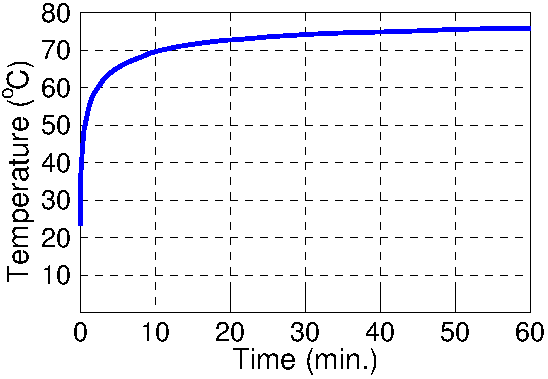
\includegraphics[width=0.45\textwidth]{YokeHeating.pdf}
	\caption{The heat distribution after $60$ minutes of beam exposure at the upstream dump location is shown. The highest 
	temperature in the yoke is at the region of the impact and is $76^\circ$C assuming an initial uniform temperature of $22^\circ$C.}
\label{fig:ansys_yoke}
\end{center}
\end{figure}





\subsection{Cryogenic target}
\label{sec-cryotgt}

Hall B experiments are grouped into running periods according to beam energy and targets. So far two types of cryogenic targets have been 
used for experiments; liquid hydrogen (LH$_2$) and liquid deuterium (LD$_2$). The Hall-B cryotarget system from the $6$ GeV era  
\cite{CLAS} has been modified for CLAS12 operation.  The current target cell is a 50-mm long Kapton cone with $23.66$ mm and $15.08$ mm upstream and downstream diameter diameters, respectively. The entrance and exit windows for the beam are a 30-$\mu$m-thick aluminum. The typical target density is $71$ mg/cm$^3$ for LH$_2$ 
and $169$ mg/cm$^3$ for LD$_2$. The cryo-liquids are sub-cooled to reduce the density variations and prevent from boiling and formation of bubbles. Figure~\ref{fig:targsch} shows the design 
rendering of the target cell inside the scattering chamber.  The scattering chamber is made of Rohacell XT110 foam (density 
$\rho=0.110$ g/cm$^3$) and is $\sim$45 cm long with a 100 mm outer diameter such that it fits within the CLAS12 silicon tracker (SVT) 
(described elsewhere in this volume) and provides a minimal material thickness for scattered particles from the target to the CLAS12 detectors.  

A beam halo monitor is integrated within the target cell. This device consists of a 40-mm-long glass cylinder with inner and outer diameters 
of 10 mm and 12 mm, respectively, mounted directly on the upstream window of the target cell with its axis parallel to the beamline and 
with 16 optical fibers attached to the upstream perimeter of the cylinder. Light generated in the cylinder 
from interactions of the beam halo or from back-scattered secondaries are readout with a multi-anode photomultiplier tube. The device, called 
the  beam-offset monitor (BOM), is used to monitor the beam position at the target (see discussion below).  

The scattering chamber extends downstream of the Central Detector. There is a 50-$\mu$m-thick aluminum window on the downstream end 
of the scattering chamber that closes the upstream vacuum beamline (from the accelerator to the CLAS12 target). The downstream vacuum 
beamline starts after a 60-cm-long air gap after the scattering chamber and ends at the beam dump.  

\begin{figure}[t]
\begin{center}
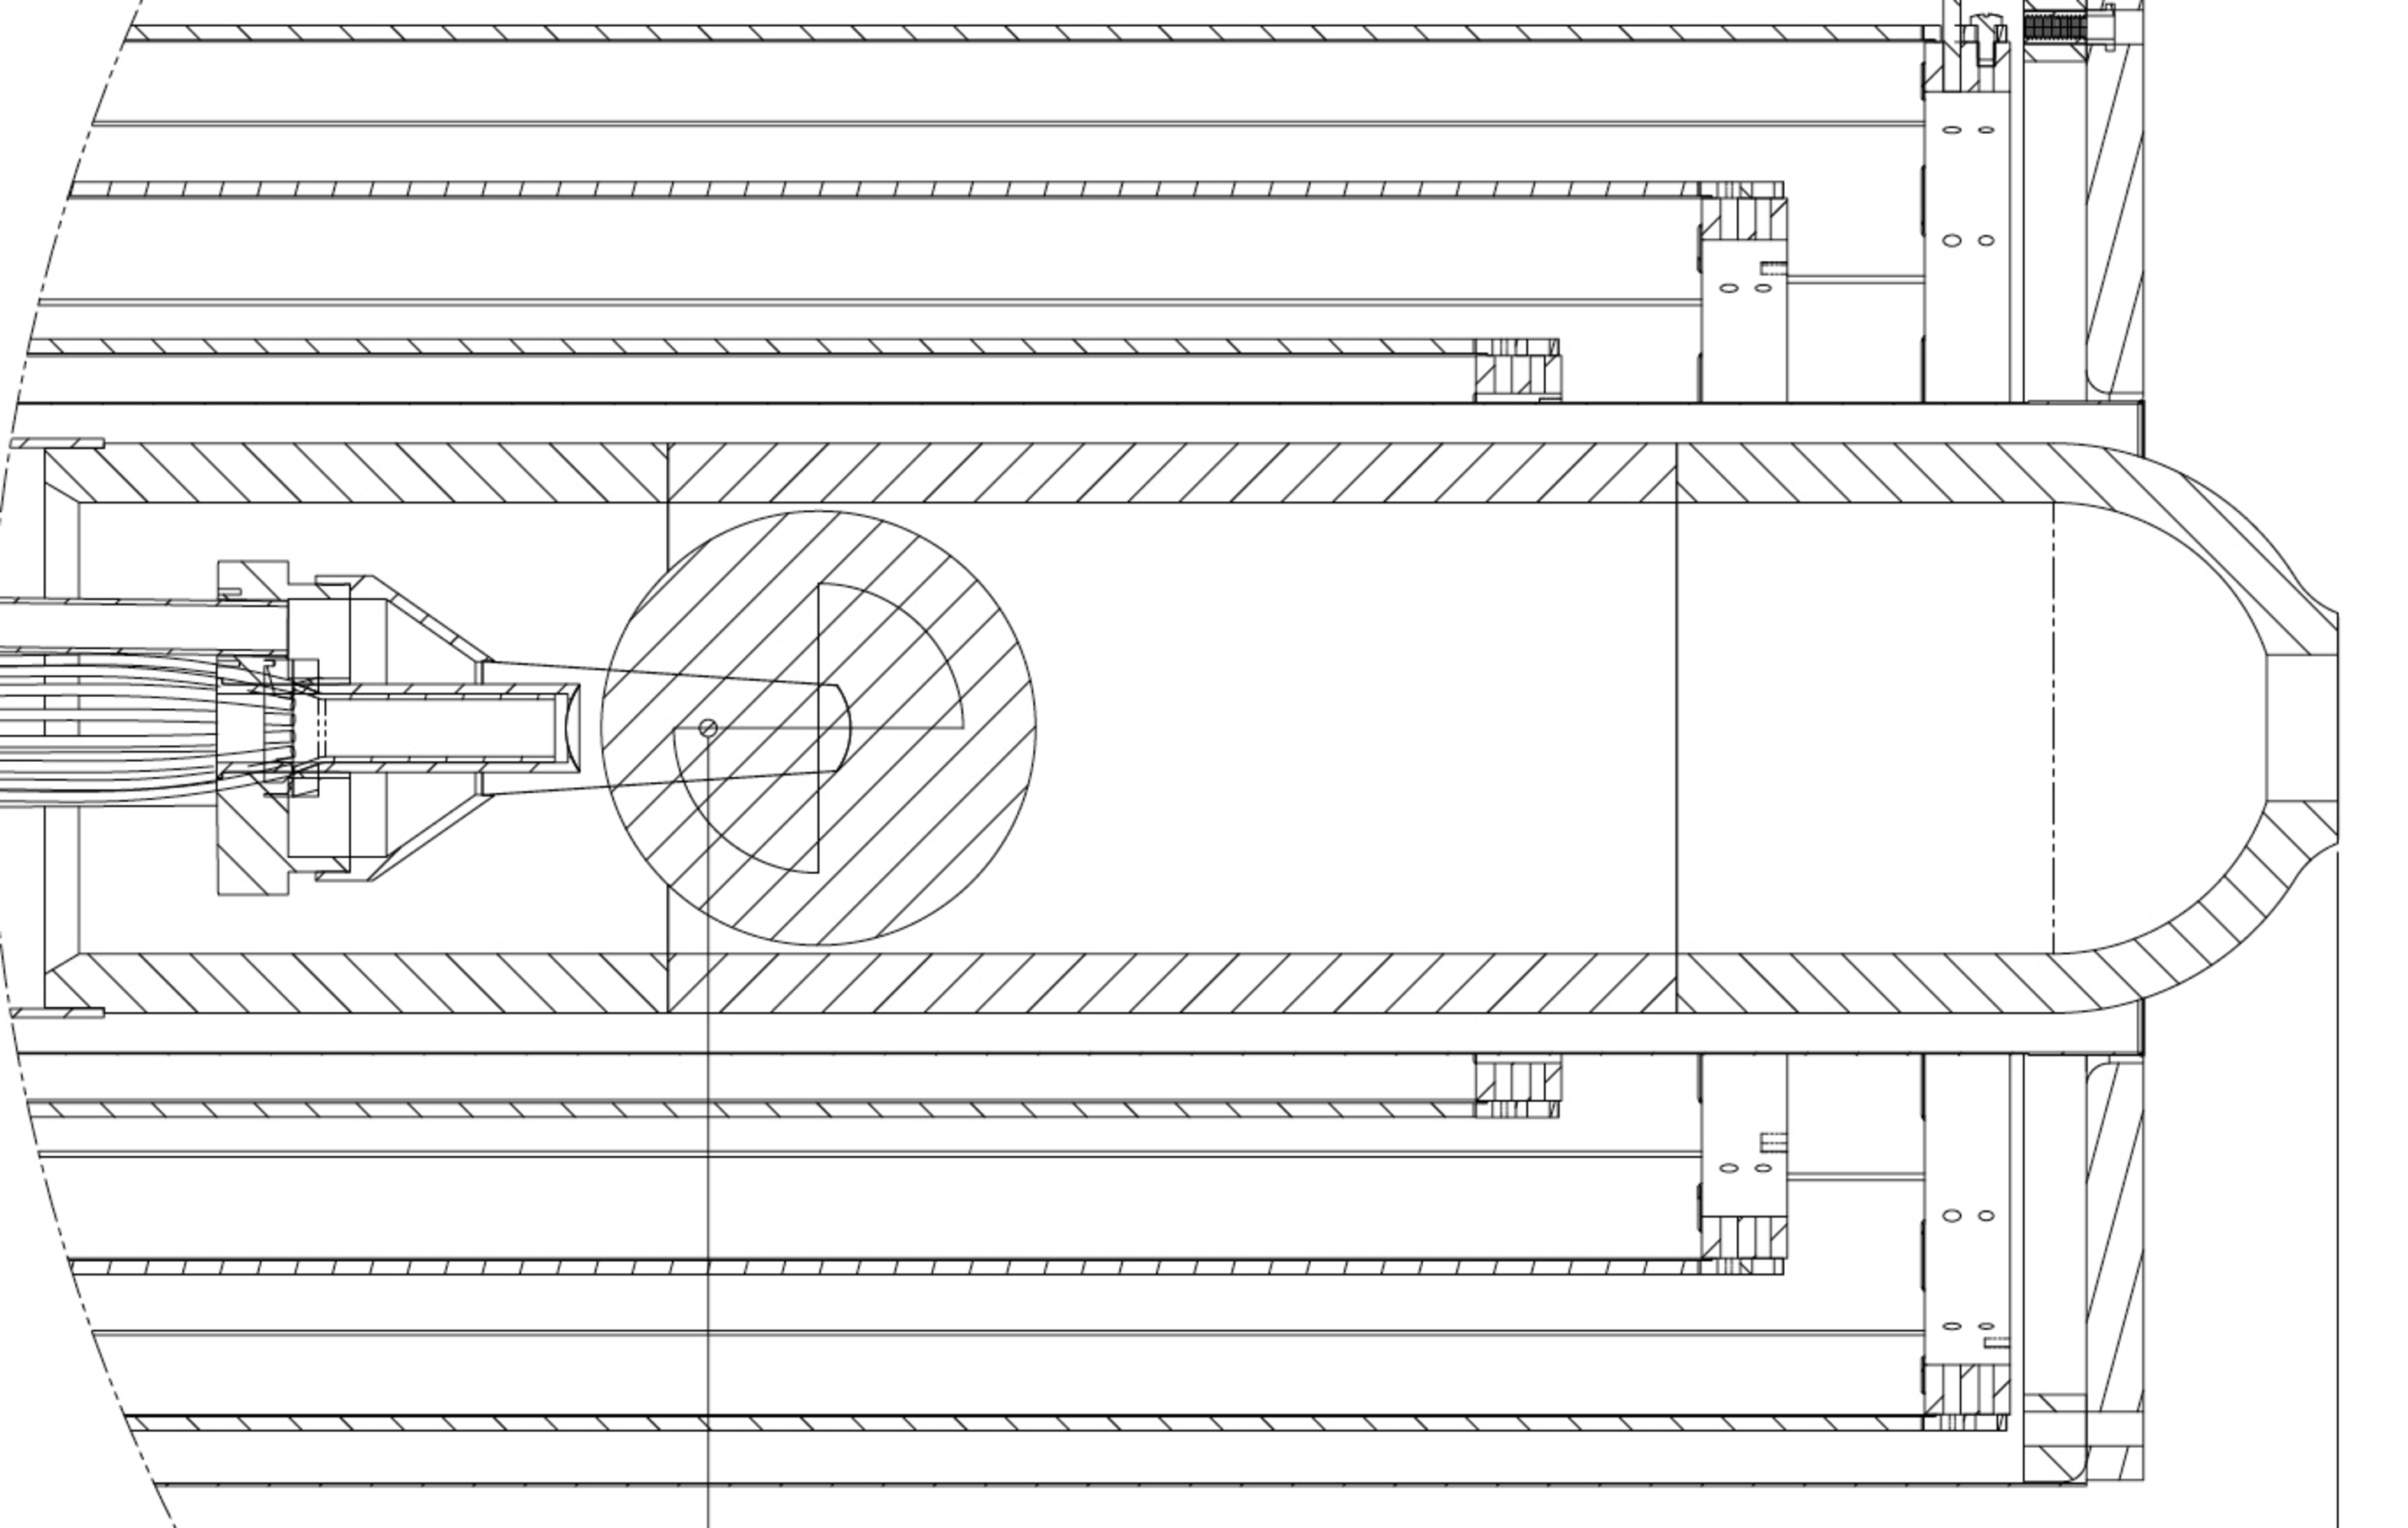
\includegraphics[width=0.45\textwidth]{target_sch.pdf}
%\includegraphics[width=0.45\textwidth]{TCell.pdf}
	\caption{Sketch of the cryogenic target showing the target cell, beam offset monitor, and scattering chamber with associated plumbing 
	and structural supports.}
\label{fig:targsch}
\end{center}
\end{figure}

\begin{figure*}[t]
\begin{center}
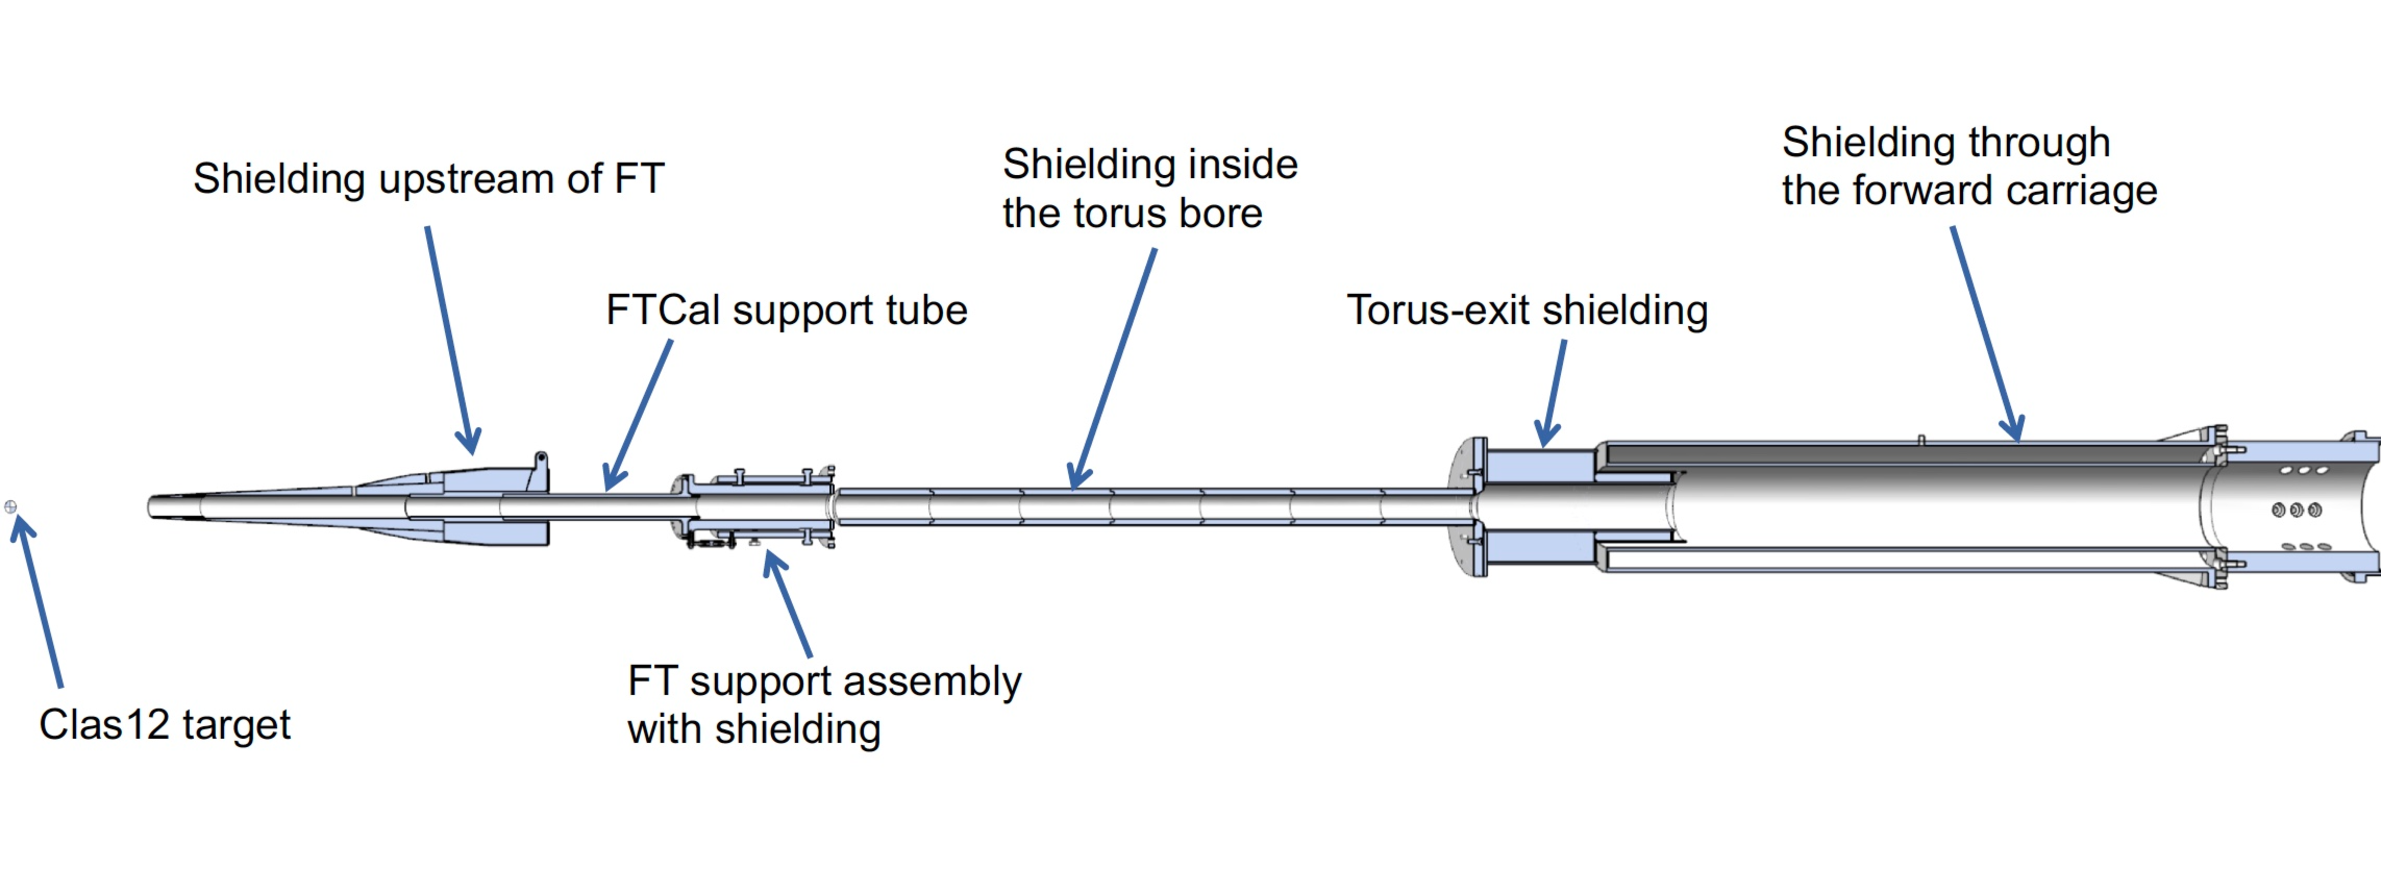
\includegraphics[width=1.\textwidth]{beamline_hall_shielding.pdf}
\caption{Tungsten shielding downstream of the target, through the torus magnet bore.}
\label{fig:shield}
\end{center}
\end{figure*}


In addition to the cryogenic targets mentioned above and already used in two experiments (LH$_2$ and LD$_2$), there will be experiments
that will use nuclear targets in the form of thin foils and experiments with polarized targets. The nuclear target assembly is similar to the 
cryogenic target cell except that various target foils will be inside the cell instead of a liquid. The cryotarget supply lines will be used to flow 
helium gas through the cell to dissipate heat in the foils from the beam. Two types of polarized targets will be used for CLAS12 experiments
\cite{Keith:2015ete}; dynamically (longitudinally) polarized ammonia (NH$_3$) and deuterated ammonia (ND$_3$), and a polarized solid 
HD target in a frozen spin mode. 

\subsection{Shielding downstream of the target} 

Special care was taken to protect the CLAS12 detectors from beam-induced background radiation. The main sources of the background are 
small-angle electron scattering along with electromagnetic processes such as bremsstrahlung, pair production, and M{\o}ller scattering. 
These interactions produce photons, electrons, and positrons that can flood the tracking detectors. GEANT4 simulations of CLAS12
have been used to study backgrounds and design appropriate shielding to reduce the levels of background radiation.  The shielding design
takes advantage of the 5-T longitudinal magnetic field around the target that is generated by the Central Detector superconducting solenoid 
magnet. This strong longitudinal magnetic field causes low-energy particles to spiral forward and away from the detectors and into the 
shielding far downstream of the target. The heavy shielding materials (lead and tungsten) contain the background and either absorb it or 
guide the flux of particles out the downstream end of CLAS12 without interacting in the detectors. 

Because CLAS12 will run with and without the Forward Tagger (FT) (described elsewhere in this volume) in use, two shielding 
configurations were designed. Figure~\ref{fig:shield} shows the configuration when the FT is in use. The shielding starts with a 
tungsten cone with a 5-cm diameter hole at the center for the beam. When the FT is in use, the tungsten cone is mounted directly 
to the FT central support, which is also made from tungsten. In this case, the angular acceptance of particles scattered from the target 
starts at $\sim 2^\circ$. For the configuration without the FT, a large diameter lead cylinder is inserted between the FT central support 
(after removing the FT tracker) and the tungsten cone, thus moving the cone closer to the target. In this case the acceptance for forward 
scattered particles starts at $\sim 5^\circ$. The shielding elements also include cylindrical tungsten absorbers inside the torus bore, a 
tungsten shield around the FT mounting fixture to the torus, and a lead-tungsten shield downstream of the torus.  

\begin{figure}[t]
\begin{center}
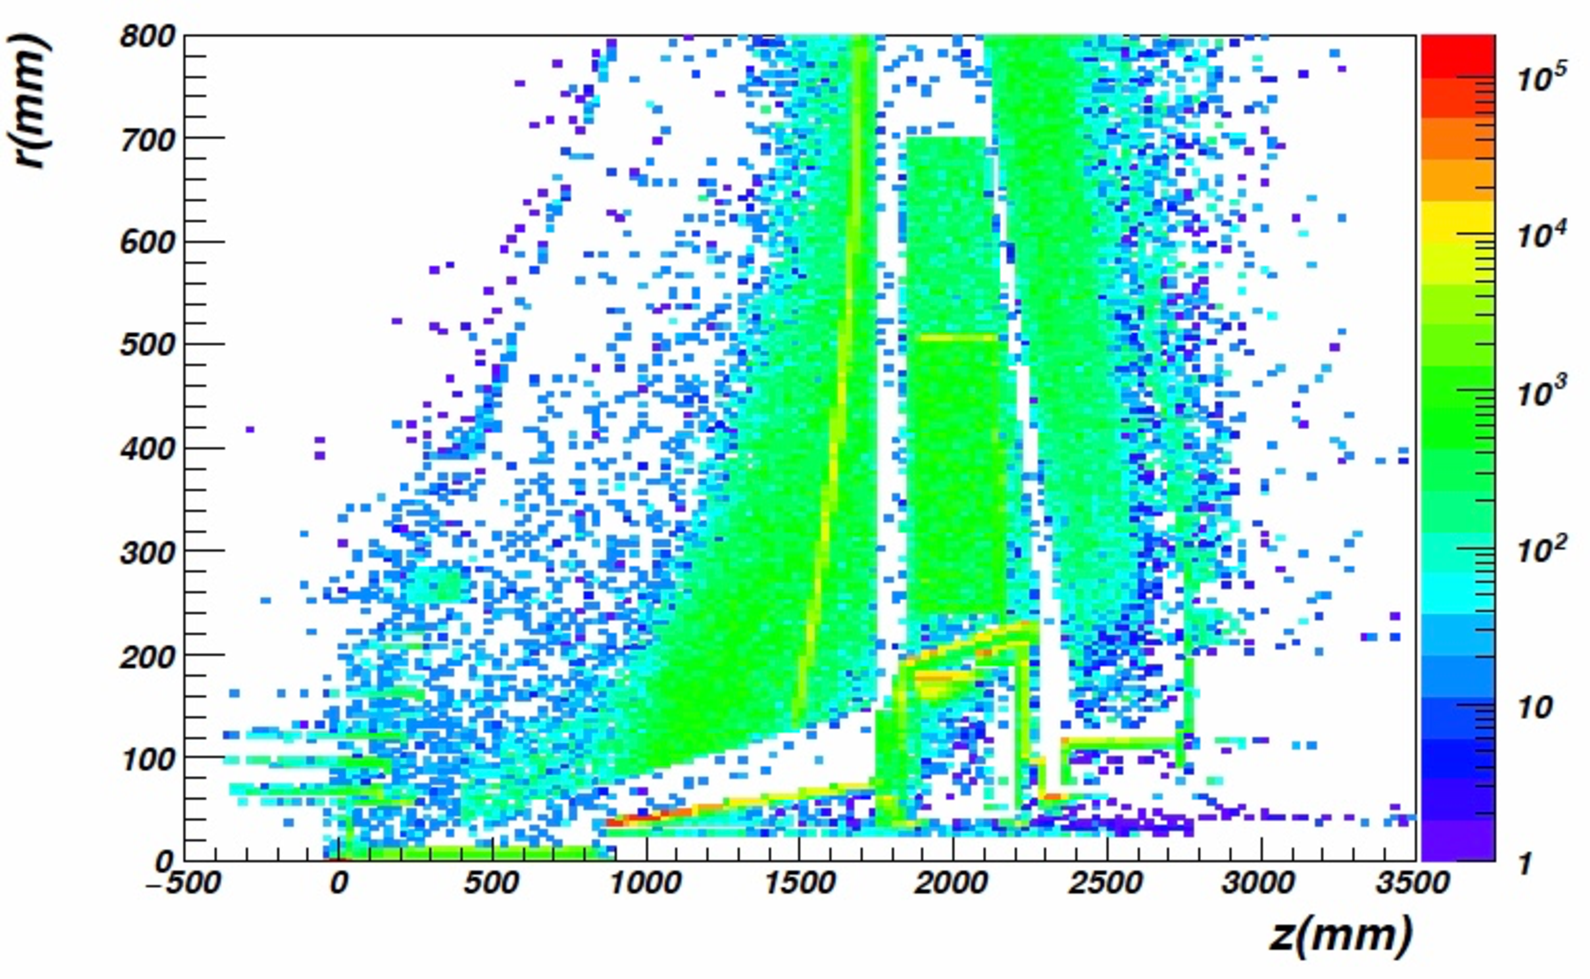
\includegraphics[width=0.48\textwidth]{fton_final_origin.pdf}
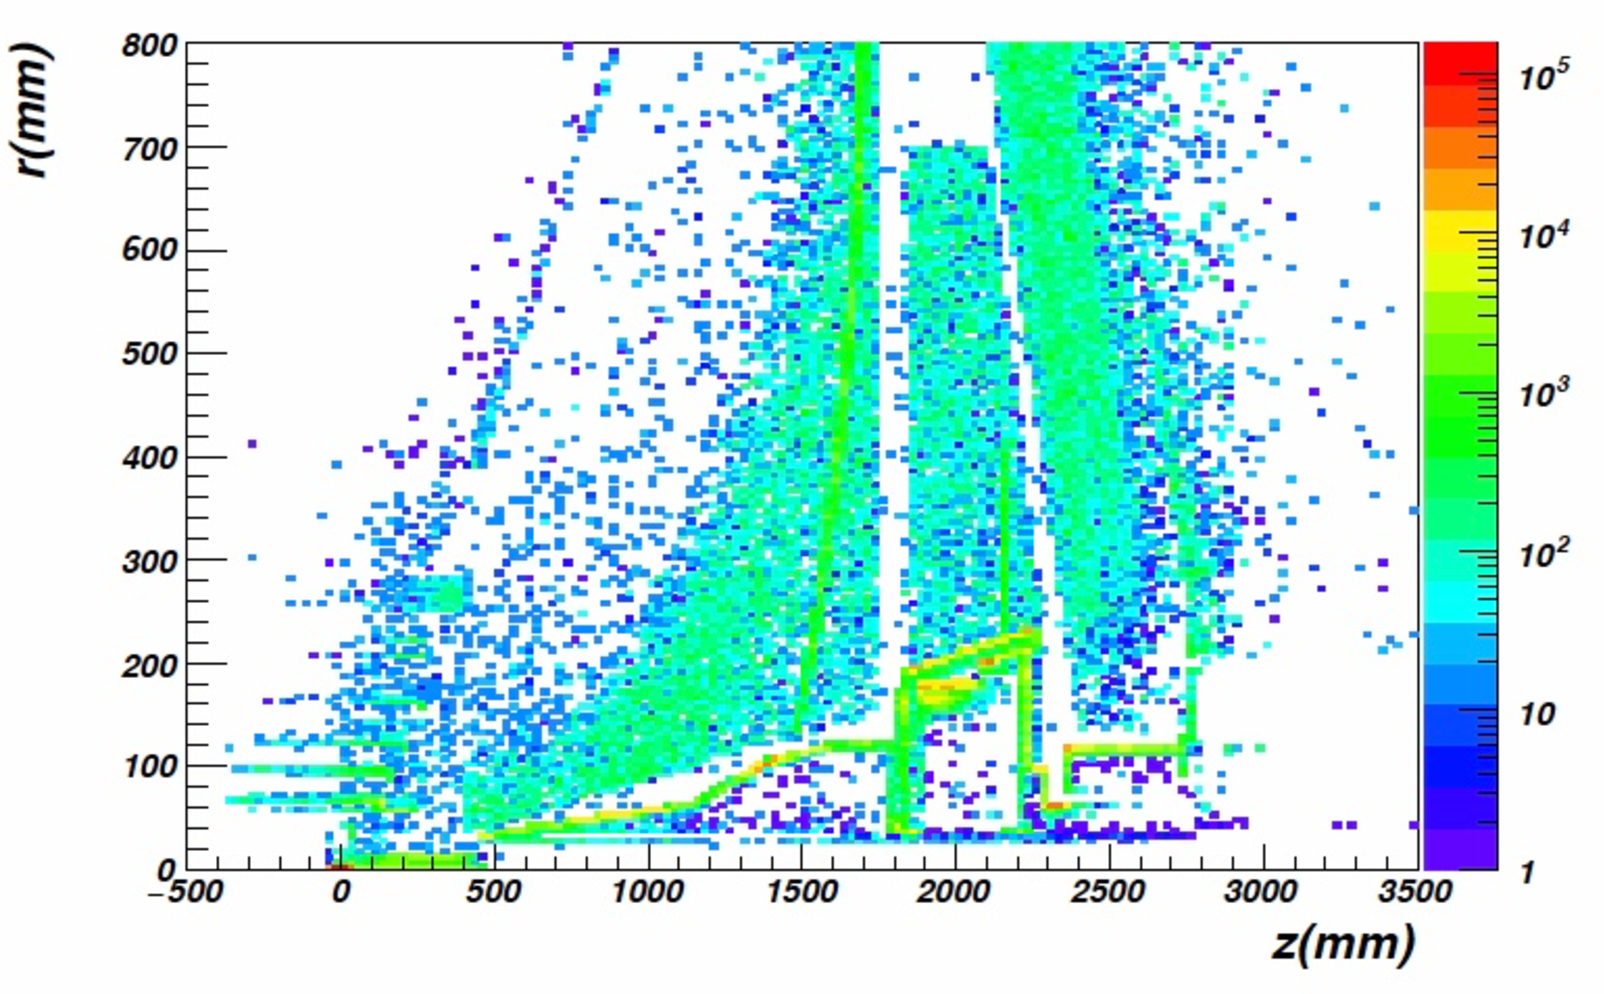
\includegraphics[width=0.48\textwidth]{ftoff_final_origin.pdf}
	\caption{The origin of particles hitting Region 1 drift chambers in the $R$-$z$ plane, where $R$ is the transverse distance from 
	the beam and the $z$ is in the beam direction. The top graph corresponds to the FT-on configuration and the bottom graph is for 
	FT-off. The main source of the background is the target located at $R=0$ and $z=0$. The second largest source is the edge of 
	the tungsten shield that starts from (40,850) and extends to (60,1700), followed by the outer edge of the Forward Tagger calorimeter 
	enclosure located around $R=200$ mm and $z=2000$ mm. The other large source is the mirror of the high-threshold Cherenkov 
	counter shown as almost vertical band at around $z=1550$ mm.}
\label{fig:origin}
\end{center}
\end{figure}

One of the main criteria for the shielding design is to maintain an occupancy rate in the drift chambers (described elsewhere in this volume)
of less than 4\% since higher occupancies adversely affect the track reconstruction efficiency.  Drift chamber occupancies were simulated 
by accumulating hits in the detector elements over 250-ns time frames, which roughly corresponds to the readout time window for the drift 
chambers. The simulated beam was spread out over this time window to match the actual beam structure and was incident on the 5-cm-long 
LH$_2$ target such that the design luminosity of $10^{35}$ cm$^{-2}$ s$^{-1}$ was achieved in the simulation. The simulated target 
included the aluminum entrance and exit foils and the air gap downstream of the target. The final shielding configuration resulted in 
occupancies of less than about 3\% for the FT-on configuration and less than about 1.5\% for the FT-off configuration.  Figure~\ref{fig:origin} 
shows the origins of background particles hitting the drift chambers for both shielding configurations. The main source of the background 
is the target with other sources being the edges of the tungsten shield, and detector enclosures (see figure caption for details). 


